% Kapitel 2 Arbeitsmittel------------------------------------------------- %
\section{Arbeitsmittel}
% ---------------------------------------------------------------------------- %
In diesem Kapitel wird der Versuchsaufbau, die Messmittel und der Messvorgang genauer erläutert.

% **************************************************************************** %
\subsection{Versuchsaufbau}
% **************************************************************************** %
Der Versuchsaufbau, wie in der Abbildung \ref{fig:Versuchsaufbau} aufgezeigt, beseht aus der Lichtquelle, dem zu messende Beugungsobjekt und einer Linse, welche auf einer Zeiss-Schiene montiert sind. Das zu beobachtenden Beugungsmuster kann am Ende der Schiene mit einer Messeinrichtung gemessen werden. Die Messeinrichtung ist auf einer Mattscheibe montiert.

\begin{figure}[h!]
	\centering
	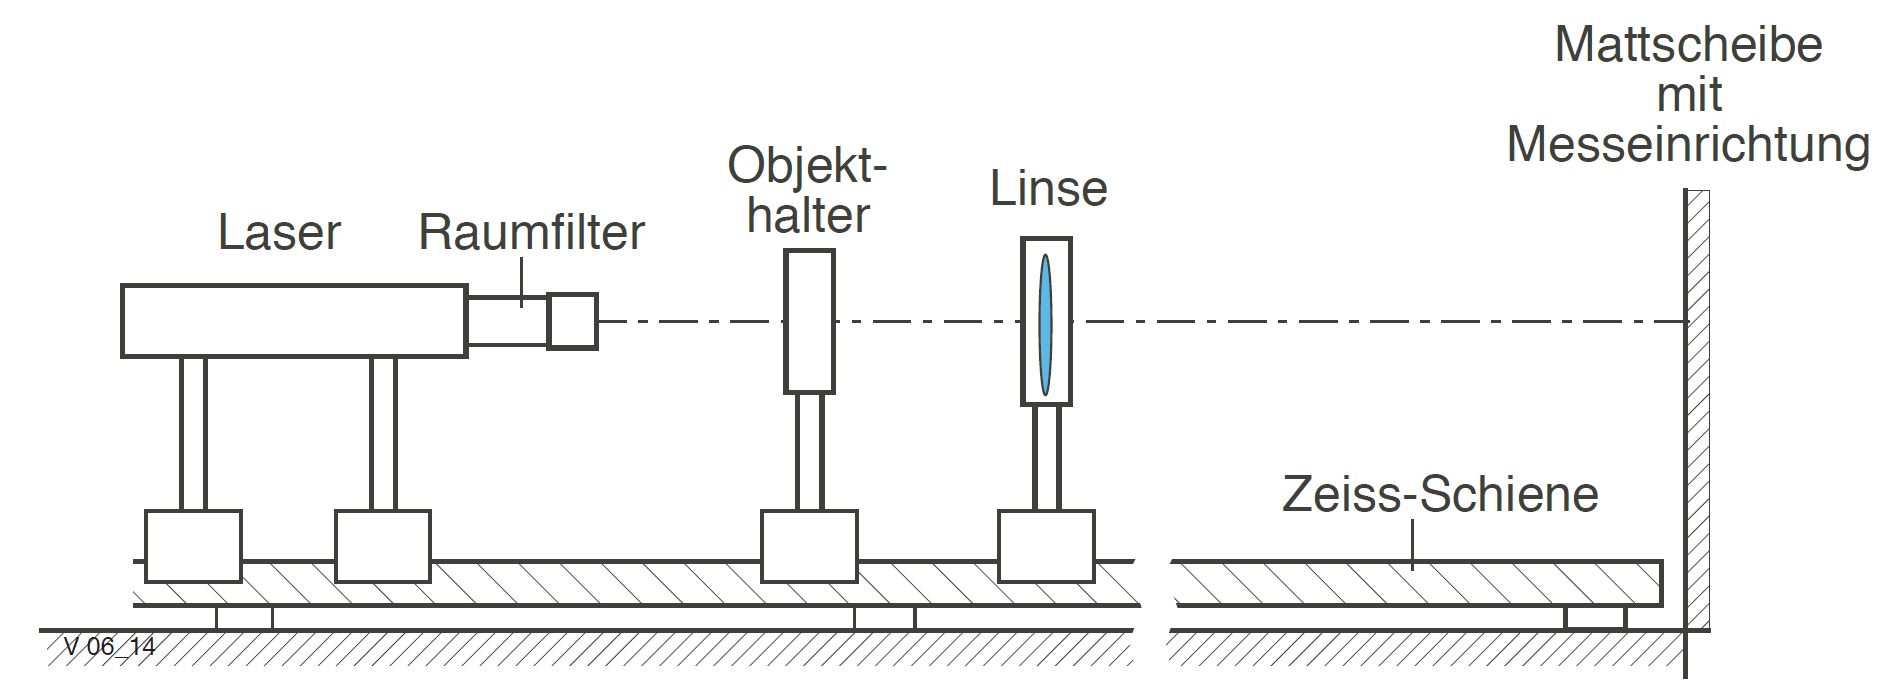
\includegraphics[width=\textwidth]{data/versuchsaufbau}
	\caption{Versuchsaufbau, des Laser, optische Elemente und der Mattscheibe}
	\label{fig:Versuchsaufbau}
\end{figure}

\begin{figure}[h!]
	\centering
	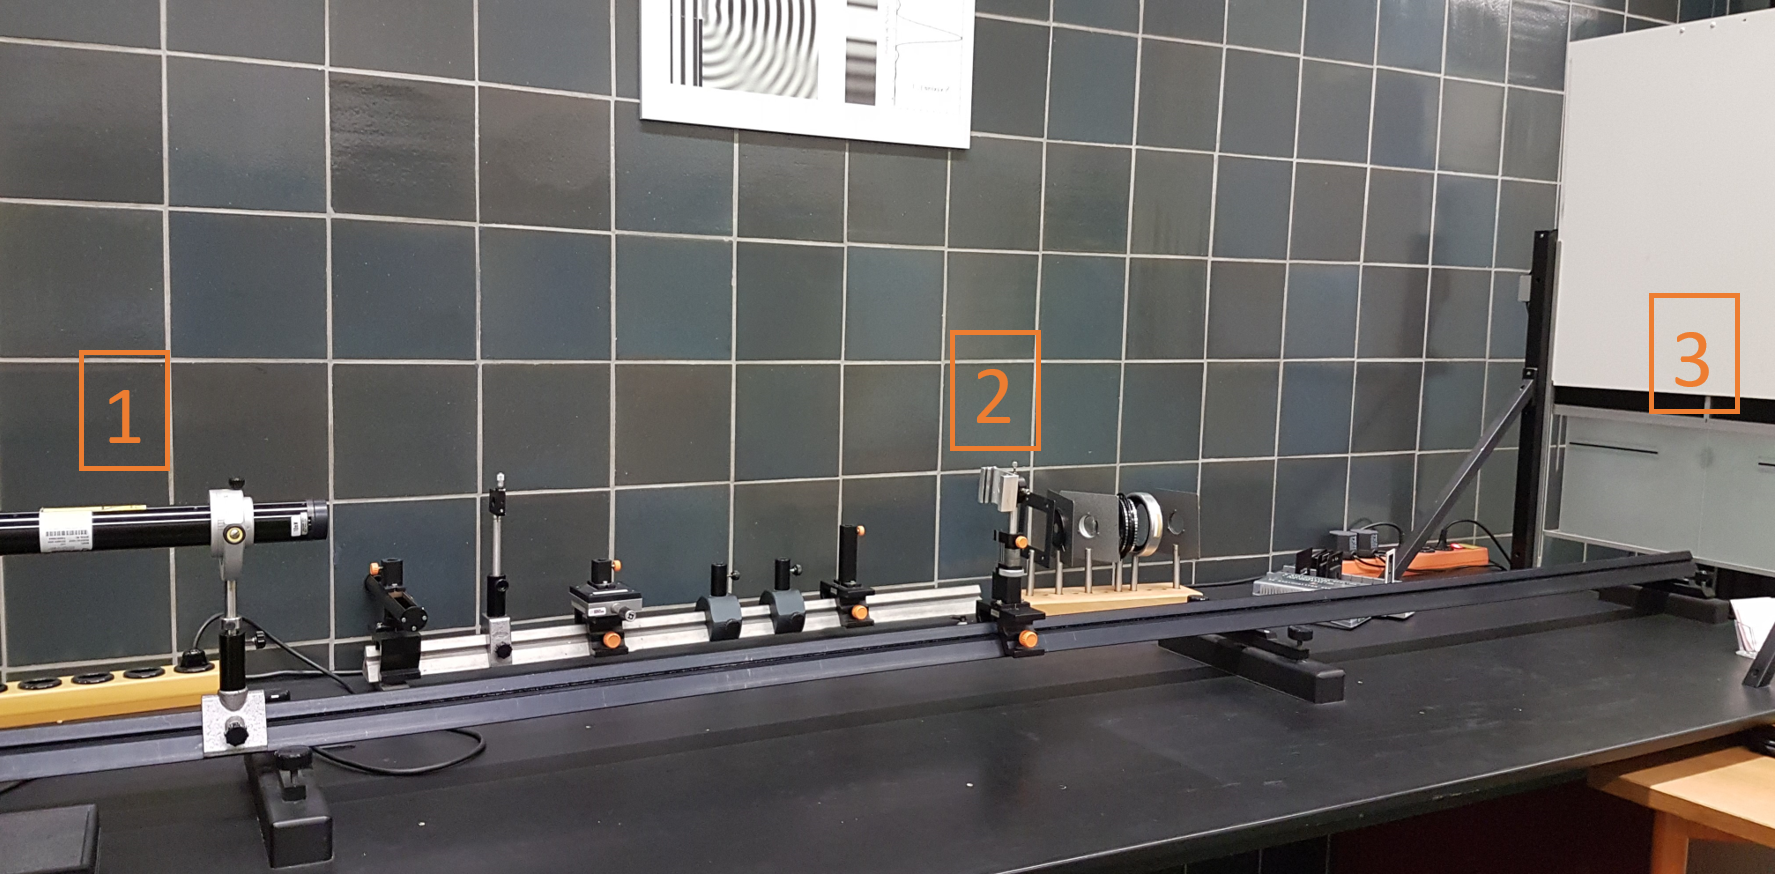
\includegraphics[width=\textwidth]{data/aufbau2}
	\caption{Versuchsaufbau mit dem Laser (1), mit dem Beugungsobjekt (2) und der Messeinrichtung (3).}
	\label{fig:org.Versuchsaufbau}
\end{figure}

% **************************************************************************** %
\subsection{Messmittel}
% **************************************************************************** %
\begin{table}[h!]
	\centering
	\begin{tabular}{|l|l|}
		\hline
		\rowcolor[rgb]{0.89,0.89,0.89}
		\textbf{Gerätebezeichnung} & \textbf{Typ}   \\ \hline
		Laser                      & He-Ne-Laser 632.8nm (rot)    \\ \hline
		Linse                      & f=2030mm                                     \\ \hline
	\end{tabular}
\caption{Messmittel die für den Versuchsaufbau genutzt wurden.}
\label{Messmittel}
\end{table}

% **************************************************************************** %
\subsection{Messobjekte}
% **************************************************************************** %
\begin{figure}[h!]
	\centering
	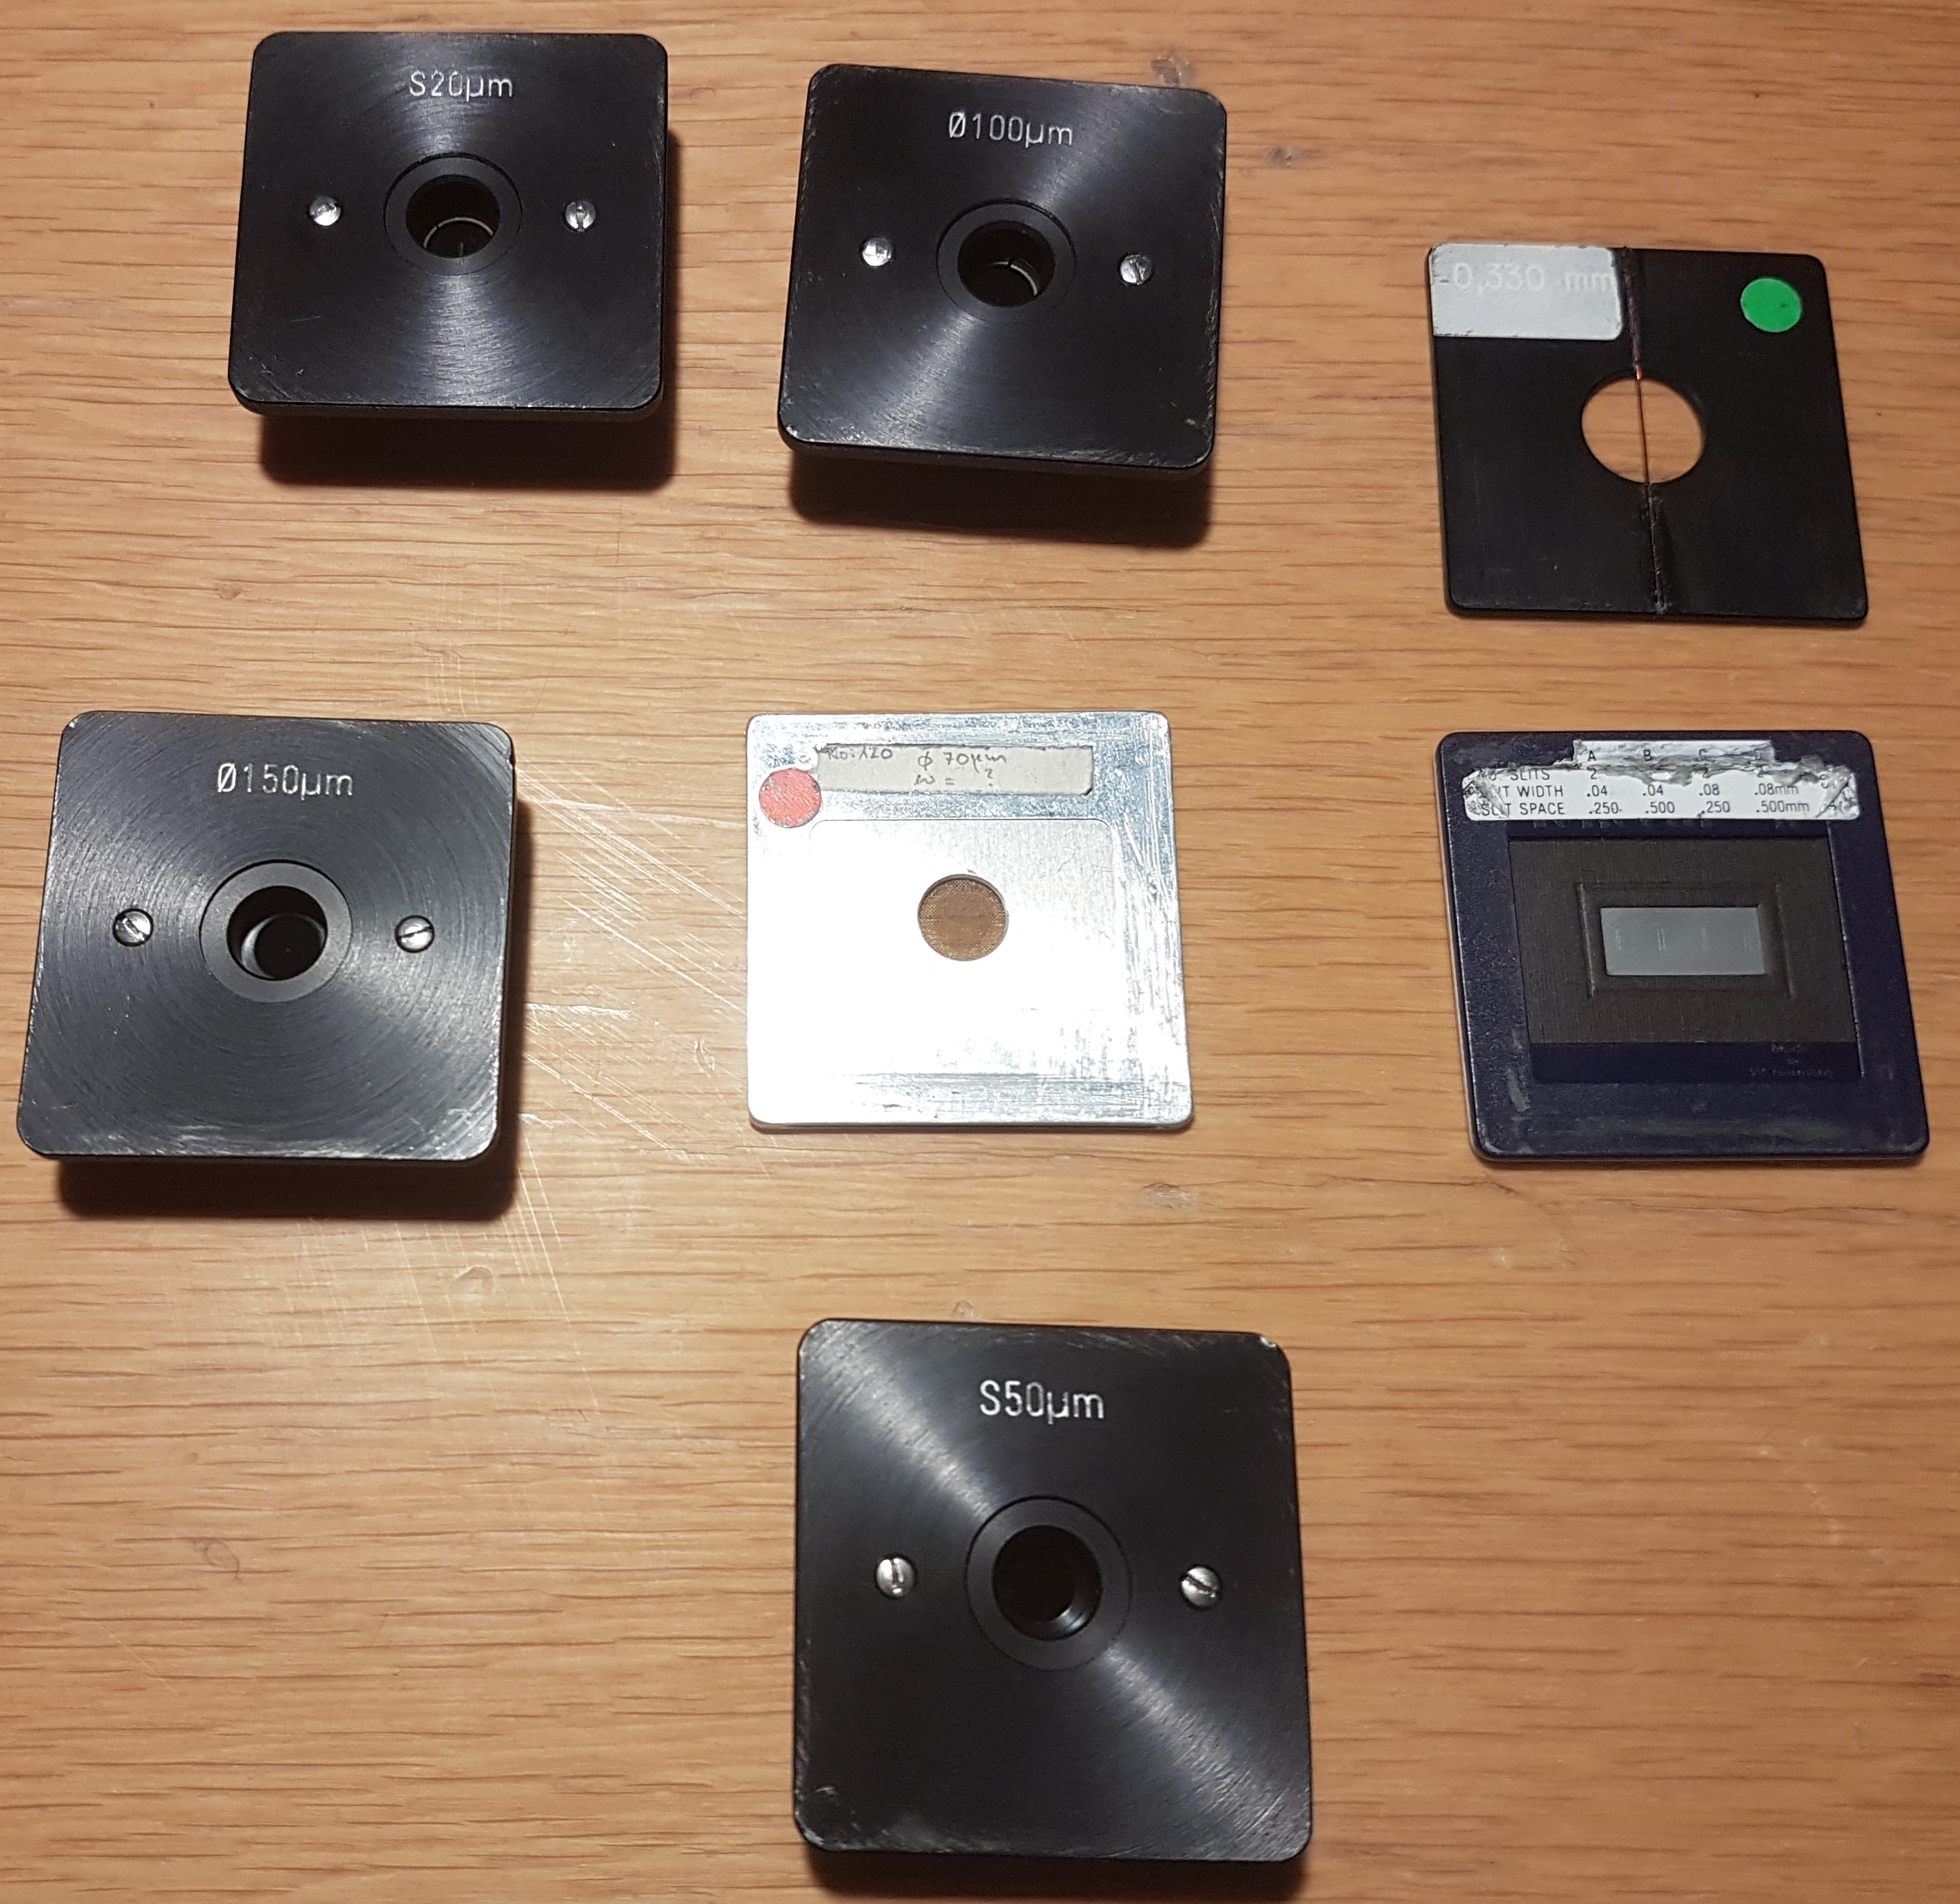
\includegraphics[width=0.6\textwidth]{data/objekte}
	\caption{Verschiedene Beugungsobjekt (Spalt, Antispalt, Loch, Gitter und Doppelspalt) die gemessen wurden}
	\label{fig:objekte}
\end{figure}

\begin{table}[h!]
	\centering
	\begin{tabular}{|l|l|}
		\hline
		\rowcolor[rgb]{0.89,0.89,0.89}
		\textbf{Typ} & \textbf{Breite}         \\ \hline
		Spalt 1      & 50    $ \cdot  10^{-6}m $    \\ \hline
		Spalt 2      & 200   $ \cdot  10^{-6}m $    \\ \hline
		Antispalt 1  & 0.33  $ \cdot  10^{-3}m $    \\ \hline
		Antispalt 2  & 0.124 $ \cdot  10^{-3}m $    \\ \hline
		Loch 1       & 150   $ \cdot  10^{-6}m $    \\ \hline
		Loch 2       & 100   $ \cdot  10^{-6}m $    \\ \hline
		Gitter       & 70    $ \cdot  10^{-6}m $    \\ \hline
		Doppelspalt  & 40    $ \cdot  10^{-6}m $    \\ \hline
	\end{tabular}
\caption{Messobjekte}
\label{table:messobjekte}
\end{table}
\newpage
% **************************************************************************** %
\subsection{Messvorgang}
% **************************************************************************** %
Bei diesem Versuch werden drei verschiedene Messungen durchgeführt. Diese Unterversuche sind:
\begin{itemize}
	\item Beugung am Spalt und Antispalt
	\item Beugung am Loch und Antiloch
	\item Beugung am Doppelspalt 
\end{itemize}

% **************************************************************************** %
\subsubsection{Beugung am Spalt und Antispalt}\label{cap:Spalt}
% **************************************************************************** %
Bei diesem Versuch werden die Abstände symmetrisch liegender Minima n-ter Ordnung bestimmt. Nach der Beugungstheorie mittels Regression kann aus diesen Werten die Breite des Spalts oder Drahtes berechnet werden. Dieser Messvorgang kann angewendet werden um den Durchmesser eines Haares oder einer Faser zu bestimmen.

\begin{figure}[h!]
	\centering
	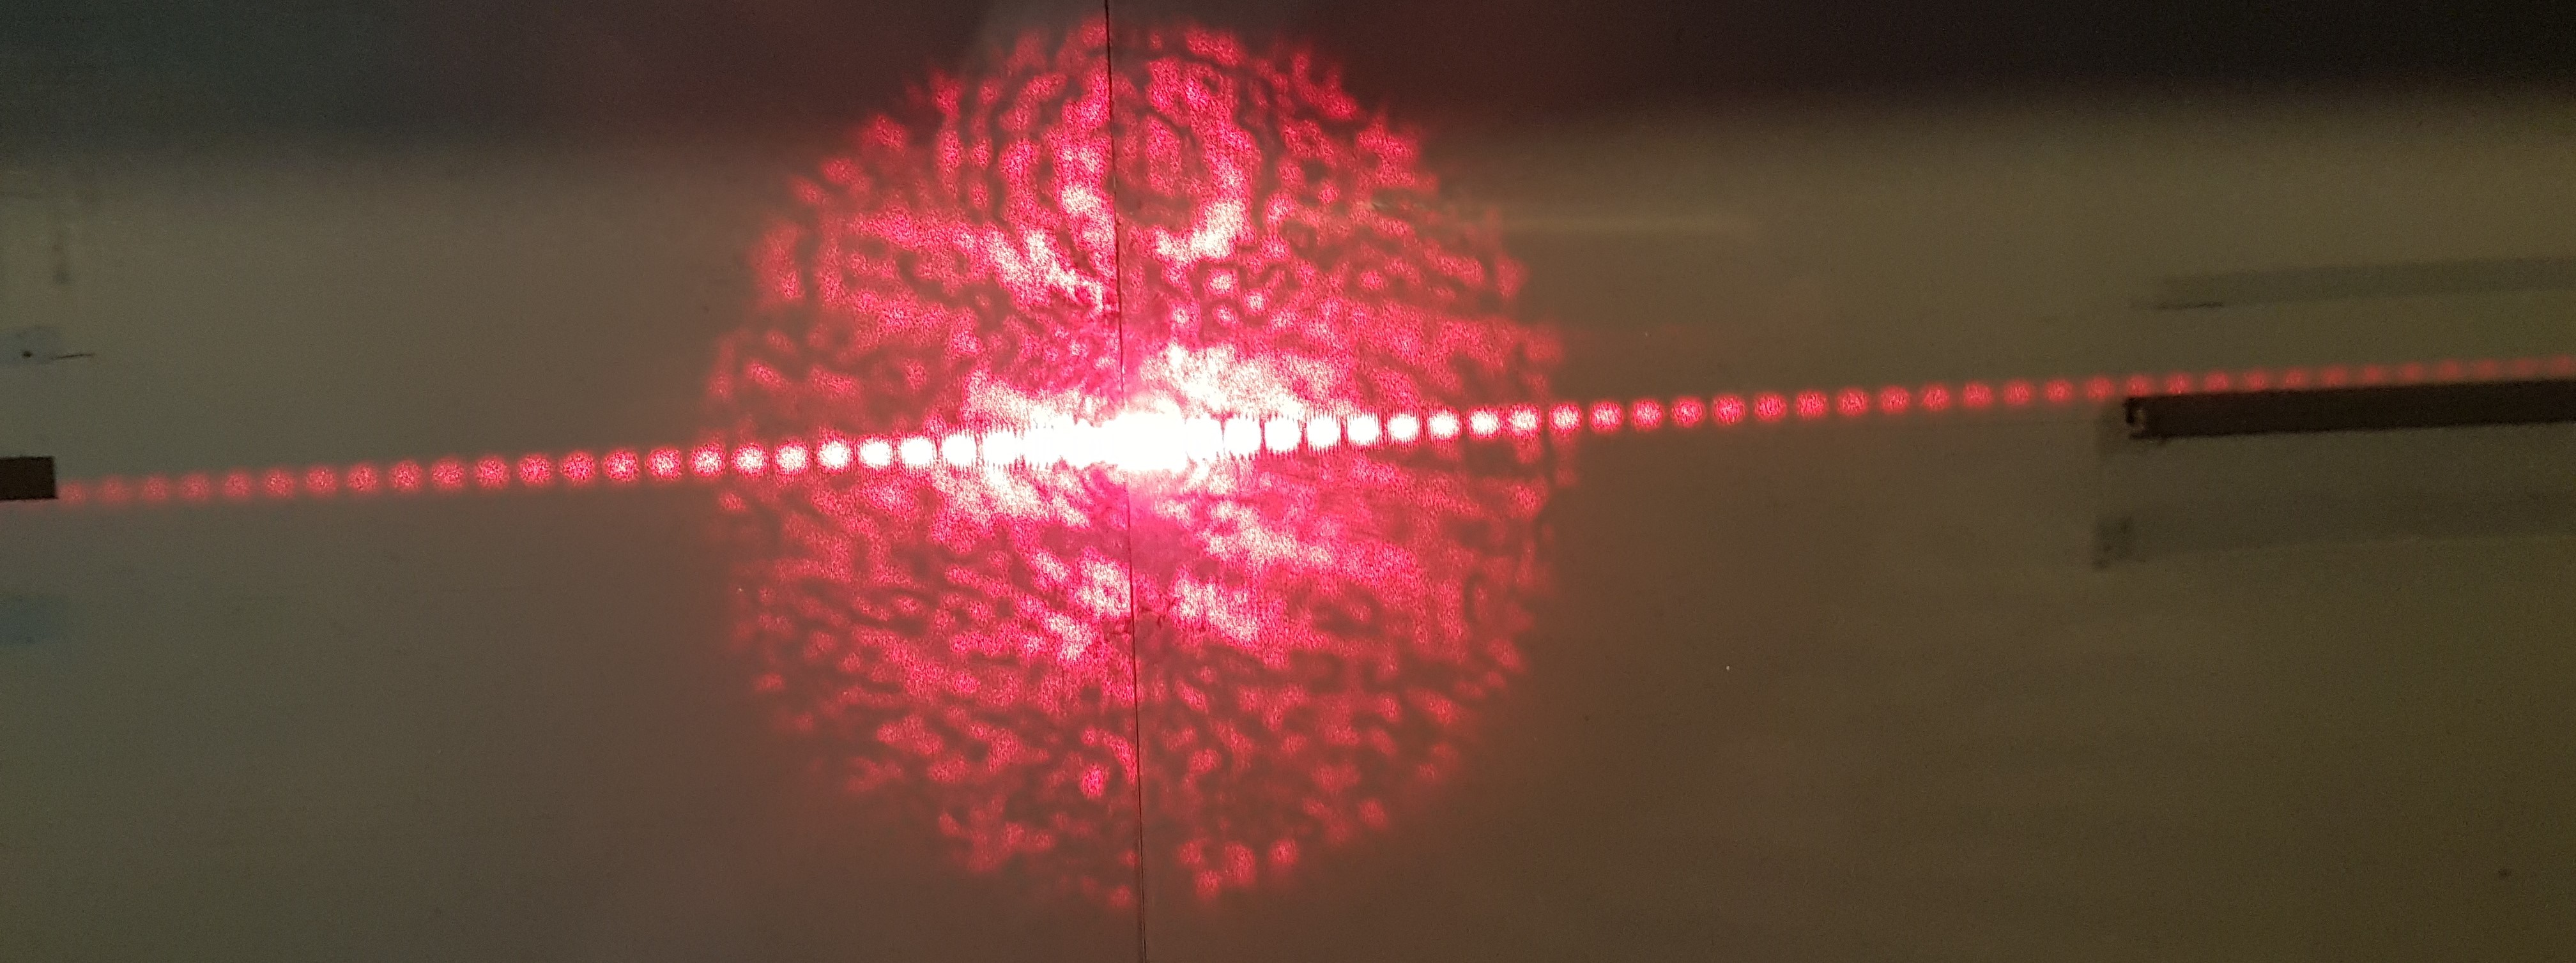
\includegraphics[width=0.5\textwidth]{data/versuch_spalt}
	\caption{Versuchsaufbau, des Laser, optische Elemente und der Mattscheibe}
	\label{fig:Versuchsaufbau}
\end{figure}

% **************************************************************************** %
\subsubsection{Beugung am Loch und Antiloch}
% **************************************************************************** %
Wie in dem Versuch \ref{cap:Spalt} wird anhand der beobachteten Minimas der Durchmesser des Loches bzw. mittleren Durchmesser der Teilchen berechnet. Wenn Pollenkörner untersucht werden, entsteht bei der Fraunhofer'scher Beobachtungsart dasselbe Interferenzmuster wie für ein einzelnes Objekt. In diesem Fall steigt die Intensität proportional zur Zahl der Beugungszentren an. Wenn sich verschiedene Interferenzmuster überlagern entsteht ein etwas verschwommenes Bild, welches dem mittleren Durchmesser entspricht.

\begin{figure}[h!]
	\centering
	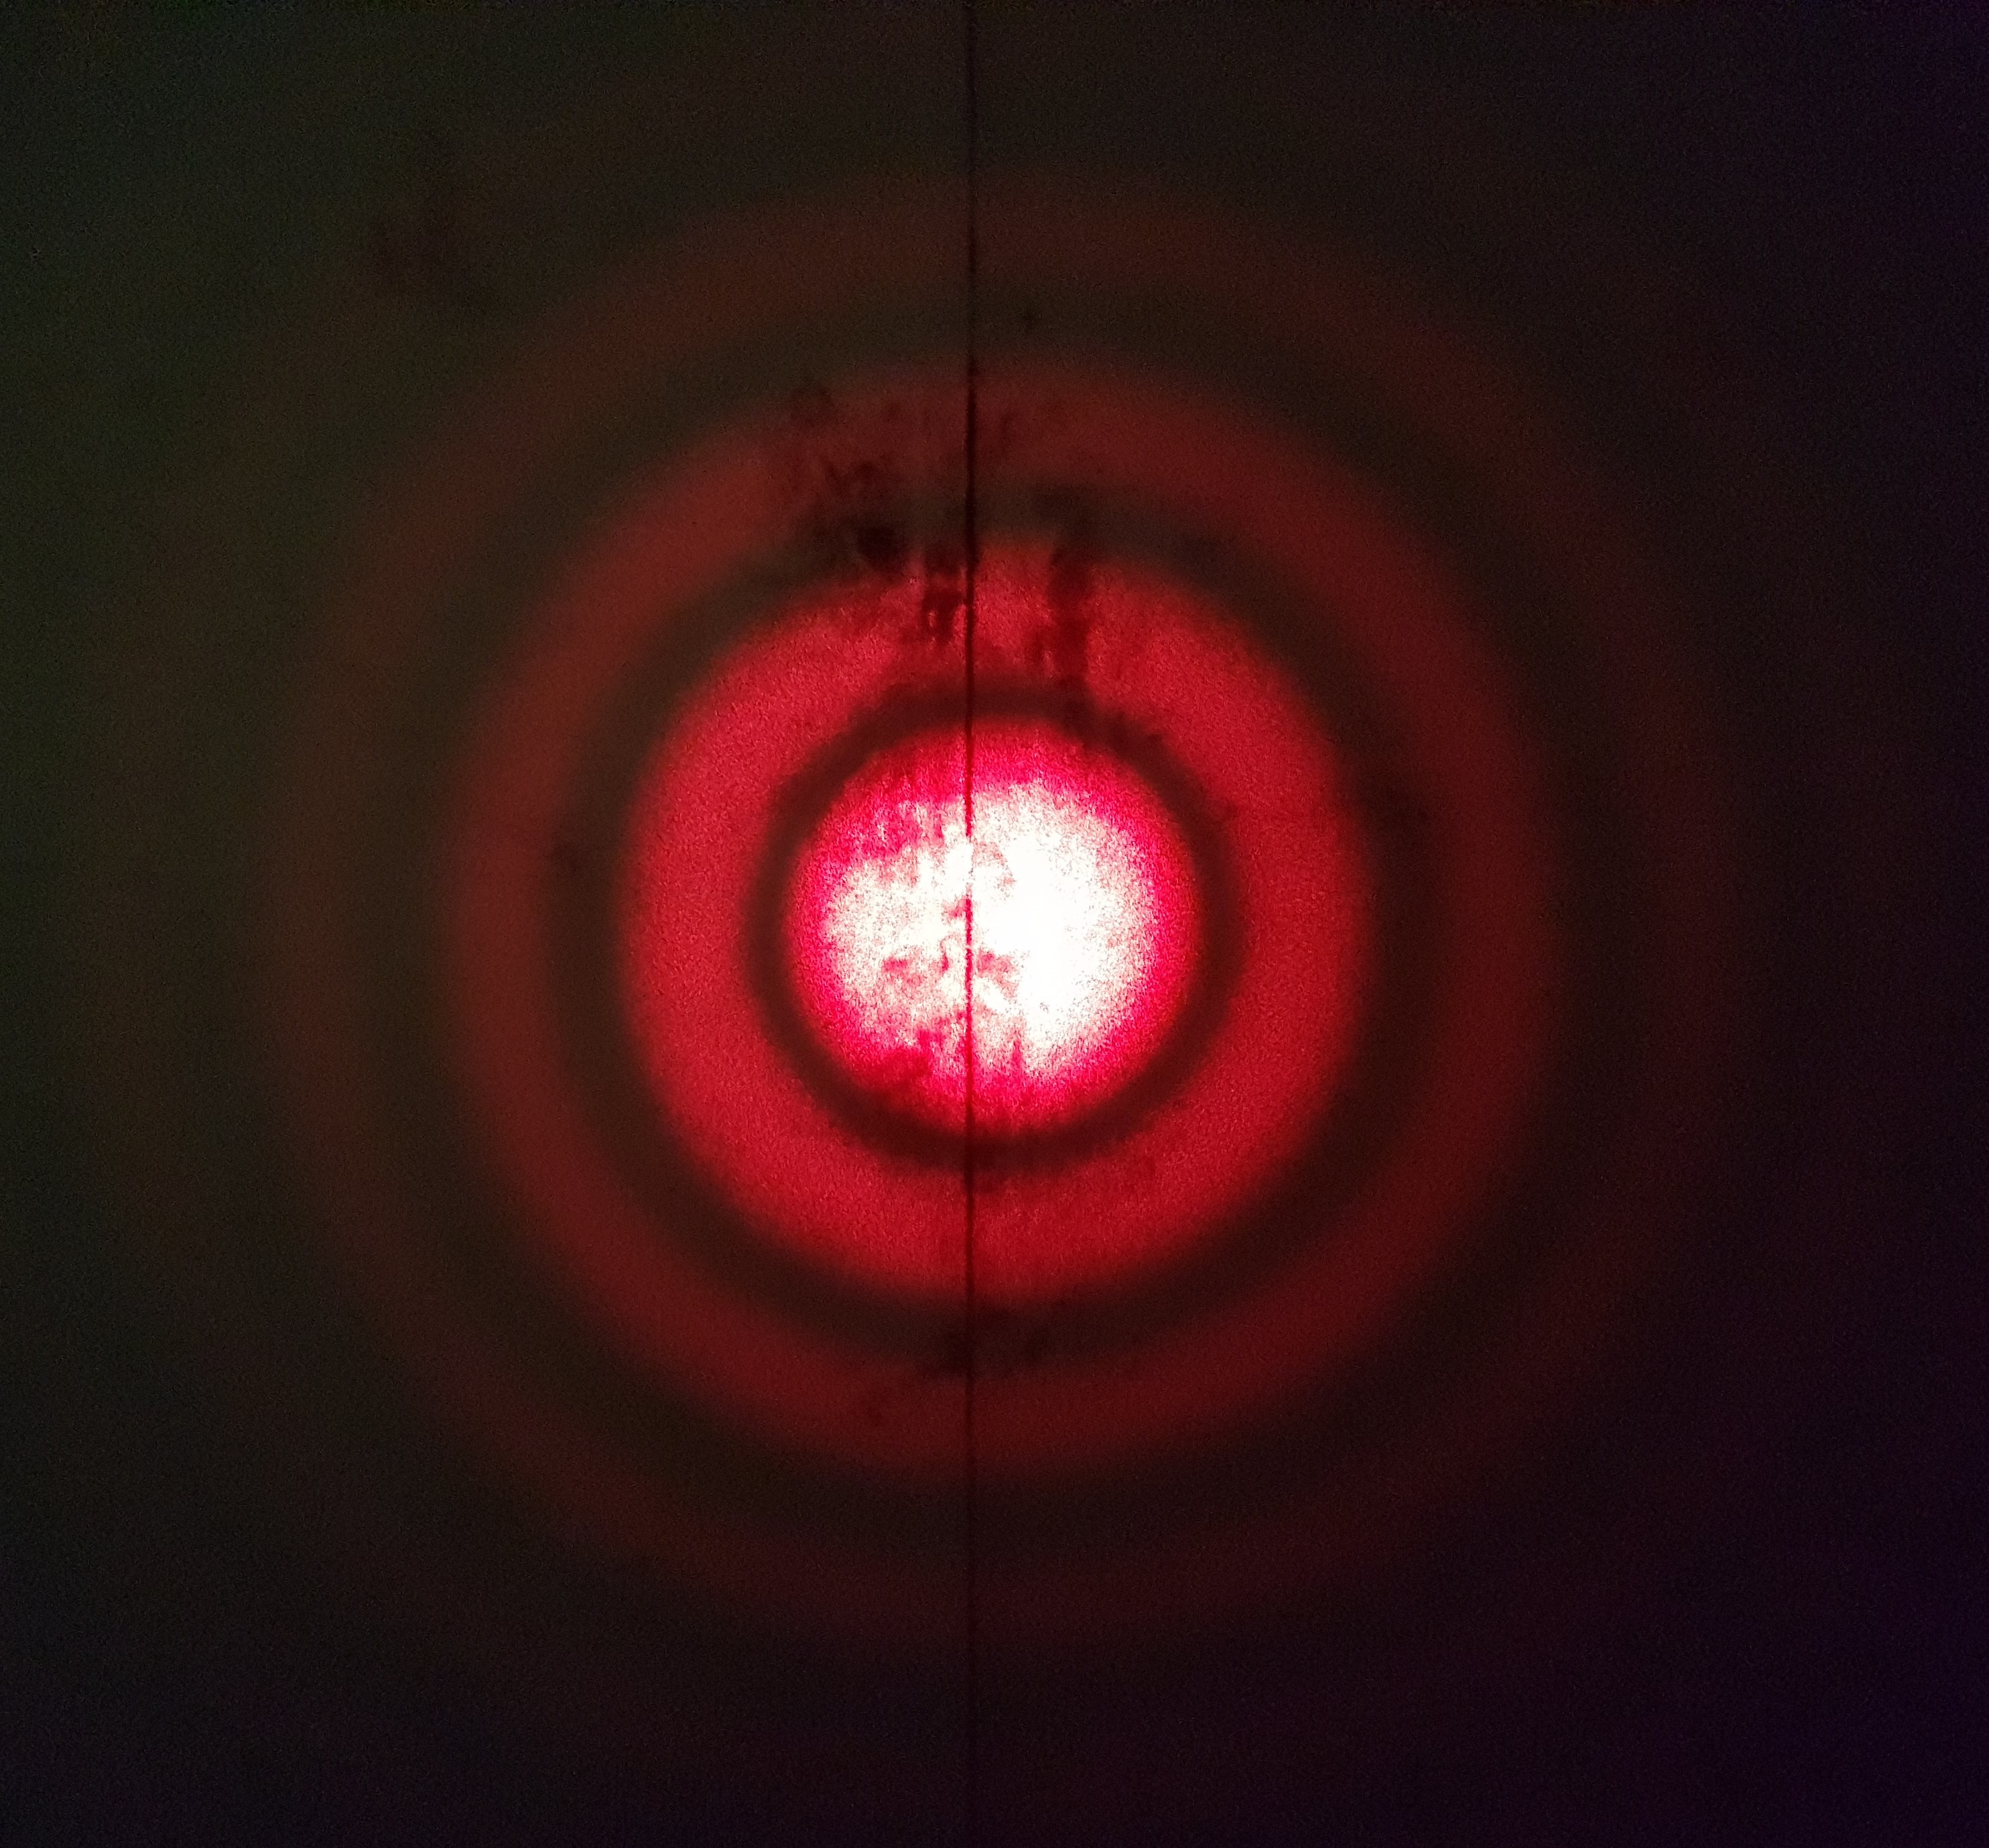
\includegraphics[width=0.5\textwidth]{data/versuch_loch}
	\caption{Versuchsaufbau, des Laser, optische Elemente und der Mattscheibe}
	\label{fig:Versuchsaufbau}
\end{figure}

% **************************************************************************** %
\subsubsection{Beugung am Doppelspalt}
% **************************************************************************** %
